\documentclass[aps,prl,twocolumn,superscriptaddress,10pt]{revtex4-1}  % for review and submission
%\documentclass[aps,twocolumn,floatfix,prl,10pt]{revtex4-1}
%\documentclass[letterpaper,10pt,prl,twocolumn,aps]{revtex4-1}
%\documentclass[aps,preprint,floatfix,prl]{revtex4-1}
\usepackage{amsmath}
\usepackage{amsfonts}
\usepackage{amssymb}
\usepackage{graphicx}
\usepackage{booktabs}
\usepackage{color}
\usepackage{longtable}
\usepackage{array}
\usepackage{amssymb}
\usepackage[usenames,dvipsnames,svgnames,table]{xcolor}

\graphicspath{ {images/}{images/Growth_Rate_Cont_Plots/} }
\newcommand{\bn}{{\boldsymbol{\hat{n}}}}
\newcommand{\bt}{{\boldsymbol{\hat{t}}}}
\newcommand{\bu}{\mathbf{u}}
\newcommand{\grad}{\mathbf{\nabla}}
\newcommand{\del}{\partial}
\newcommand{\hg}{h_g}
\newcommand{\Rey}{\text{R}}
\newcommand{\Ndg}{\tilde{N}_g}
\newcommand{\monami}{\textit{monami }}
% \newcommand{\shreyas}[1]{{\bf (#1)}}
\newcommand{\shreyas}[1]{}
\definecolor{tableShade}{gray}{0.8}

\begin{document}
\title{The onset of of hydrodynamically driven waving of marine grass in flow}
\author{Ravi Singh}
\affiliation{Brown University, Providence RI 02912 USA}
\author{L. Mahadevan}
\affiliation{Harvard University, Cambridge MA 02138 USA}
\author{M. M. Bandi\thanks{work performed while visiting Brown University}}
\affiliation{Collective Interactions Unit, OIST Graduate University, 1919-1 Tancha, Onna-son, Okinawa, Japan 904-0495}
\author{Amala Mahadevan}
\affiliation{Woods Hold Institute of Oceanography, Woods Hole MA USA}
\author{Shreyas Mandre}
\affiliation{Brown University, Providence RI 02912 USA}

\begin{abstract}
We show that the threshold flow condition for the spontaneous waving of marine grass arises due to the drag exerted by the vegetation on the flow. 
We show this by developing a self-consistent model of the flow past rigid vegetation. 
Linear stability analysis of the steady flow resulting from this model naturally leads to the threshold condition, and explains its mechanistic origin. 
Asymptotic analysis of the model for dense grass reveals two unstable modes. 
One of these modes shares many common features with the Kelvin-Helmholtz instability, but is demonstrated to be different from it. 
The predictions of the model for threshold condition and the resulting dominant frequency of waving agree with laboratory observations. 
\end{abstract}
\maketitle
%\section{Introduction}
Sea grasses exhibit a rich set of dynamical behavior due to their collective interaction with both steady and oscillatory flows.  
The resulting changes in hydrodynamic conditions can influence number of environmental processes such as transport of sediments, contaminants, dissolved oxygen, plant growth, and biomass production \cite{Fonseca87,Grizzle96,Nepf99,Nepf2012}. 
The simplest response of these flexible grass canopies to steady currents is the formation of coherent large amplitude oscillations, known as \monami \cite{AckermanOkubo93}.  
In this letter we provide a hydrodynamic mechanism for the onset of these coherent oscillations.
\newline
Current explanations of \monami invoke the existence of a shear layer near the top of the canopy \cite{Ghisal02,Raupach96} and its instability through a mechanism similar to the Kelvin-Helmholtz instability. 
This instability is thought to lead to coherent eddies over the sea grass canopy which then drives large amplitude synchronous oscillations.
\newline
While the shear layer model appears to predict the frequency of \monami consistent with experimental observations, several aspect of existing theory remain unsatisfactory. 
(i) While the free shear layer is established due to the vegetation drag, linear stability analysis\cite{Raupach96} does not account for this, rendering this explanation inconsistent. 
(ii) Classical free shear flow is known to be unstable for all Reynolds number\cite{drazin}, whereas observations in the lab\cite{Ghisal02} and the field\cite{Grizzle96} indicate the existence of a threshold 
flow speed below which \monami is not observed. 
(iii)The thickness of the free shear layer, defined as the momentum thickness of the boundary layer near the grass tip, is in many cases comparable to the unvegetated layer thickness,
and therefore inconsistent with the assumptions of the free shear layer instability.
Here we present a self-consistent mathematical model that account correctly for these effects 
while also explaining lab experiments and field observations.
%Using this model, the synchronous waving may be understood to be arising from the linear hydrodynamic instability of a uniform flow over the grass bed, such that the principal role of the vegetation is to exert a drag on the flow. 
%A threshold flow speed arises naturally for the onset of the instability; this threshold condition and the resulting waving frequency compares well with experimental observations.
%The vegetation drag introduces a damping mechanism in the flow, in addition to the viscous damping, and overcoming this damping is the primary consideration that sets the threshold flow.
%We deduce this numerically and through an asymptotic scaling analysis in the limit of dense grass.
\newline
The drag exerted by the grass bed on the flow is central to the hypothesized mechanism\cite{Ghisal02} of the instability underlying \monami because it realizes the shear layer structure of the flow. 
The flexibility of the grass blades, on the other hand, serves merely to aid in visualizing the flow structure resulting from the instability\cite{Nepf2012}. 
It has been demonstrated that the instability and the resulting flow structures are present even when the grass blades are replaced with rigid dowels\cite{Ghisal02}. 
Therefore, for simplicity, we consider the grass bed to form a rigid structure that exchanges momentum with the surrounding fluid but does not deform. 
Indeed, a more detailed calculation undertaken for terrestrial grass demonstrated\cite{Delangre06} that when the timescale of the instability is well-separated from the period of natural oscillations of the grass bed, 
the flow instability is similar to the instability of a shear layer. 
%\begin{figure}
%\begin{center}
%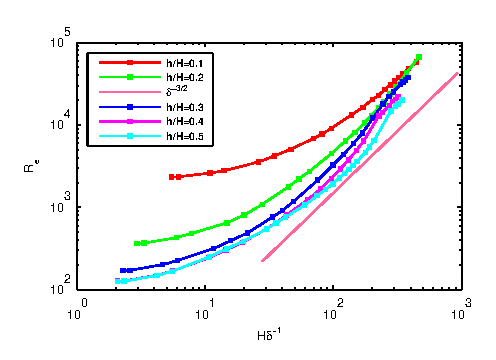
\includegraphics[]{Critical_Re_vs_delta_noshear} \\
%\vspace{-6mm} \hspace{-3mm}
%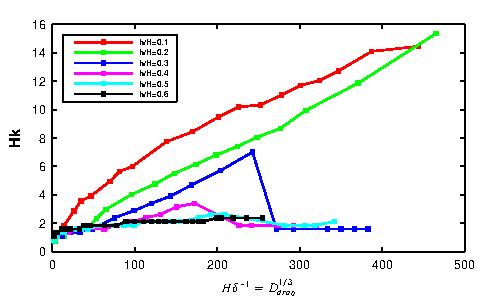
\includegraphics[]{K_vs_shear_width_noshear}
%\end{center}
%\caption{Critical Reynolds number with flow (top) and the corresponding marginally stable wave number (bottom) for different submergence ratio as a function of vegetation density
% parametrized by the boundary layer thickness. Parameters estimated from experiments reported by Ghisalberti and Nepf\cite{Ghisal02} to exhibit or suppress synchronous waving are 
%also included in the top panel. Inset compares experimental observations 
%of the dominant frequency $f_o$ (in Hz) measured with the predictions from the solution of \eqref{Orr-somerfield}. The %experimental data in the inset in obtained from publications by 
%Ghisalberti and Nepf \cite{Ghisal02} and Vivoni \cite{Vivoni98}. In order to estimate the $\Rey$ for these experiments, a %representative value of $\mu=0.1$ Pa~s was assumed.}
%\label{Re_vs_delta}
%\end{figure}
We use a mean field model for the coupling between the flow and the canopy. 
The force exerted by the grass is approximated via a continuous body force $\mathbf{f}=-N_g\mathbf{f_d}$,  
where $\mathbf{f_{d}}$ is drag force per unit length of the grass blade, $N_g$ the grass number density per unit area\cite{Vivoni98,Nepf99,Ghisal02,Delangre04,Delangre06}. 
In the canopy the equations of continuity and momentum balance can be written as 
%in the fluid momentum balance\cite{Vivoni98,Nepf99,Ghisal02,Delangre04,Delangre06} as
\begin{equation}
\quad \grad\cdot\bu = 0,\hspace{3mm} \rho \left(\bu_{t}+\bu.\grad\bu \right) = -\grad P+\mu\grad^{2}\bu +\mathbf{f}+\rho\mathbf{g}
\label{navier-stokes}
\end{equation}
%where $\mathbf{f_{d}}$ is drag force per unit length of the grass blade, $N_g$ the grass number density per unit area, 
where $\rho$ the fluid density, $\mathbf{u}$ the velocity, 
$P$ the pressure, $\mu$ the turbulent viscosity and $\mathbf{g}$ the acceleration due to gravity. 
The Reynolds number of the flow based on the scale of a grass blade is expected to be O($10^2$-$10^3$), and hence the drag force is dominated by pressure and modeled as 
$\mathbf{f_{d}}=C_N \rho u_{N}^{2}d\bn + C_{T}\rho u_{T}^{2}d\bt$ \shreyas{citation needed} 
where $d$ is average width of grass blade $C_{N}$ and $C_{T}$ are the normal and tangential drag coefficients respectively; $u_{T}$, $u_{N}$ are velocity components along and
normal to grass while $\bt,\bn$ being unit vector along and normal to grass. 
We expect $C_T \ll C_N$ and take $C_T=0$ for rest of analysis. 
In the field, both $C_N$ and $N_g$ vary with distance from the bottom but we do not expect these variation to be central to the mechanism and therefore take $C_N$ and $N_g$ to be constants. 
Based on previous experiments\cite{Vivoni98}, we take $C_N \approx 1$.
\newline
To understand the onset of \monami, we first calculate the steady flow $\bu = U(y)\boldsymbol{\hat{x}}$ as a solution of \eqref{navier-stokes}, and examine its linear stability. 
Such a steady state flow driven by constant pressure gradient satisfies 
\begin{equation}
 -\frac{dP}{dx}+\mu U''(y) +S(y) \rho C_N d N_gU^2=0
\label{base_equ}
\end{equation}
where $S(y)=1$ in the vegetated layer $0<y<\hg$ and $S(y)=0$ in the unvegetated layer $\hg< y< 2H$. 
In the limit of large grass density, shear stress exerted by the bottom surface is estimated to be negligible in comparison with the vegetation drag and hence the bottom surface ($y=0$) is approximated by zero shear.   
A comparison of the steady flow profile from the solution of \eqref{base_equ} with experimental measurements is shown in figure~\ref{basicflow}.
Flow within grass has approximately constant velocity $U_g \sim \sqrt{\frac{dP/dx}{\rho C_N dN_g}}$ arising from the balance between drag and with pressure gradient, and the flow outside has a simple parabolic velocity profile due to the balance between viscous forces and the pressure gradient. 
Continuity of flow speed and shear stresses at canopy top gives rise to a boundary layer near the tip of the grass.
\begin{figure}
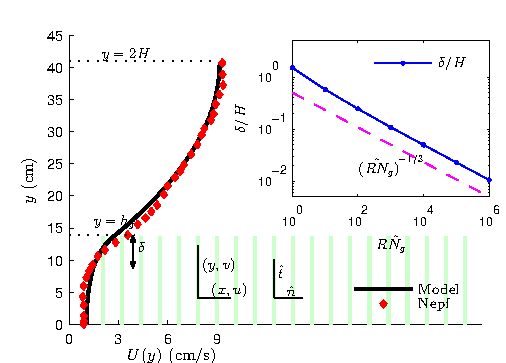
\includegraphics[scale=1]{Grass_Base_Nepf_shear}
\caption{Comparison of steady flow profile from the experiments by Ghisalberti and Nepf\cite{Nepf04} (Case-I from Table-1 with 1250 plants/m$^2$, 
plant height = 13.7$\pm 0.2$ cm and blade width of 0.64 cm)
 and it's approximation with $U_0=7.28$ cm/s and $\delta = 5.02$ cm with our model. The canopy extends upto $y=h_g$ in the water column of depth $2H$. 
The steady velocity profile can be decomposed into three regions, (i) A parabolic profile in the unvegetated region, (ii) a uniform profile deep within the grass bed, and (iii) a boundary layer of thickness $\delta$ near the canopy top. 
The dependence of the boundary layer thickness (estimated numerically as $|U/U_y|$ at $y=\hg$) on the vegetation density parameter $\Rey \Ndg$ is shown in the inset.}
\label{basicflow}
\end{figure}
This boundary layer near the canopy top results from purely local dynamics independent of the influence of the boundaries, and we identify it as a free shear layer\cite{Ghisal02} in the previous explanation of \monami. 
In our model the balance between viscous forces and the drag force in the shear layer $(\mu u_\text{sl}/\delta^2 \sim \rho C_N d N_g u_\text{sl}^2)$ and the continuity of shear stress across the grass tip $(u_\text{sl}/\delta \sim U_0/H)$, leads to a shear layer thickness $\delta=(\Rey\tilde{N_g})^{-1/3}H$, where $\Ndg = \left(C_N d H N_g\right)$ is the vegetation frontal area per bed area, $\Rey=\rho U_0 H/\mu$ is the Reynolds number of the flow, $u_{sl}$ is the velocity scale in shear layer and $U_0 = {(dP/dx)~H^2}/{\mu}$ is the velocity scale in the unvegetated region. 
This dependence of the boundary layer thickness on the grass density $N_g$, shown in Figure \ref{basicflow}, gives us a way to systematically investigate its effect on the instability mechanism.
The asymptotic regime of a thin boundary layer is expected to hold for $\Rey \Ndg \gtrsim 100$; minor departures from this scaling can be seen in the inset of figure \ref{basicflow}.
\newline
To understand the evolution of small perturbations to the steady flow profile, we substitute $\bu = (U+\tilde{u}, \tilde{v})$, $p=P+\tilde{p}$ in \eqref{navier-stokes} and expand to linear order to obtain (after dropping the tilde decoration)
\begin{equation}
\begin{split}
\rho(u_t+U u_x+vU_y) &= -p_x+ {\mu}\nabla^2u-2S\rho C_{N}dN_{g}Uu, \\
\rho(v_t+ Uv_x) &= -p_y+ {\mu}\nabla^2v, \hspace{0.3cm} \nabla\cdot\bu=0.
\end{split}
\end{equation}
These equations can be non-dimensionalized using half channel height $H$, velocity $U_0$, and the associated advection time $H/U_0$. 
We are left with three non-dimensional parameters in the model, ie. $\Rey$, $\Ndg$, and the submergence ratio of the grass $h_g/H$. 
We also use $\delta/H$ in lieu of $\Ndg$ to parametrize the grass density and help elucidate the mechanism of the instability. 
With these scaling, and using a stream function $\psi$ with $u = \psi_{y}, v= -\psi_x$ to satisfy mass balance, we seek a wave solution of 
the form $\left(u,v,\psi \right)= \left(\hat u(y), \hat v(y), \hat\phi(y) \right)e^{ikx+\sigma t}$ to  obtain a modified Orr-Sommerfield equation. 
The growth rate $\sigma$ for a given wave number $k=2\pi /\lambda$ satisfies the eigenvalue problem.
% provides growth rate and frequency associated with a perturbation of wavelength $2\pi/k$ through the solution of
\begin{figure}
\begin{center}
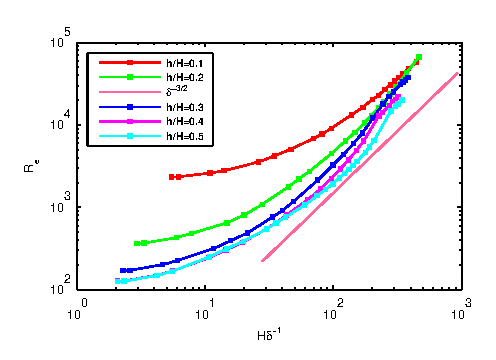
\includegraphics[]{Critical_Re_vs_delta_noshear} \\
\vspace{-6mm} \hspace{-3mm}
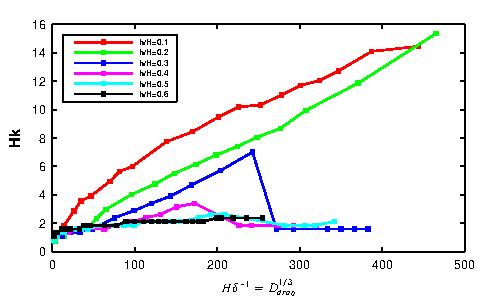
\includegraphics[]{K_vs_shear_width_noshear}
\end{center}
\caption{Critical Reynolds number with flow (top) and the corresponding marginally stable wave number (bottom) for different submergence ratio as a function of vegetation density
 parametrized by the boundary layer thickness. Parameters estimated from experiments reported by Ghisalberti and Nepf\cite{Ghisal02} to exhibit or suppress synchronous waving are 
also included in the top panel. Inset compares experimental observations 
of the dominant frequency $f_o$ (in Hz) measured with the predictions from the solution of \eqref{Orr-somerfield}. The experimental data in the inset in obtained from publications by 
Ghisalberti and Nepf \cite{Ghisal02} and Vivoni \cite{Vivoni98}. In order to estimate the $\Rey$ for these experiments, a representative value of $\mu=0.1$ Pa~s was assumed.}
\label{Re_vs_delta}
\end{figure}
\begin{equation}
\begin{split}
\left(D^2 -k^{2} \right)^2\phi &= \Rey \left[ \left({\sigma}+ikU\right) \left(D^2-k^2\right) -ikU_{yy}\right]\phi \\
&+D\left(2R \Ndg S U D \phi\right),
\label{Orr-somerfield}
\end{split}
\end{equation}
where $D=d/dy$, and subject to the boundary conditions $D\phi = D^2\phi = 0$ at $y=0$ and $y=2$. 

%We solve this eigenvalue problem 
%and in fig\ref{Re_vs_delta} we plot the frequency (Im$(\sigma)$) of the fastest growing mode with that of experimental observations of frequencies in
%the lab scale experiments, for cases where the vegetation was sufficiently dense to be modeled by a continuum drag field. 
%The observed frequencies are associated with the peaks in velocity spectra, frequency of $\monami$ and frequency of 
%vortex passage \cite{Ghisal02}, and compare well with the predicted frequencies. 

We solve this eigenvalue problem and a threshold in $\Rey$ of O(100), above which the flow is unstable (Re($\sigma$)$>$0), emerges from the 
solution of \eqref{Orr-somerfield}. The dependence of this critical $\Rey$, and the corresponding fastest growing wavenumber $k$, on $\delta/H$ and $\hg/H$ is shown 
in figure \ref{Re_vs_delta}, and is found to compare well with experimental observations\cite{Ghisal02}.
The threshold Reynolds number increases with the grass density, indicating a competition between the 
destabilizing shear in the flow, and the stabilizing effect of damping due to vegetation drag.
Previous linear stability calculations for terrestrial grass do not exhibit a threshold flow condition 
either due to the exclusion of the vegetation drag in their model\cite{Raupach96}, or because of ad-hoc
assumptions for the mean velocity profile\cite{Raupach96,Delangre06}.


\begin{figure*}
\begin{tabular}{cccc}
{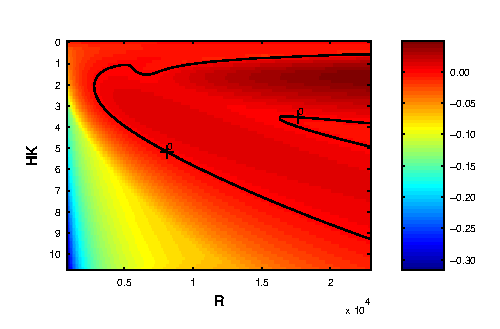
\includegraphics[scale = 0.67]{Set4_dens28_imgsc}} &
{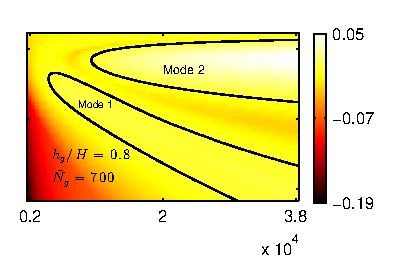
\includegraphics[scale = 0.67]{Set4_dens30_imgsc}} &
{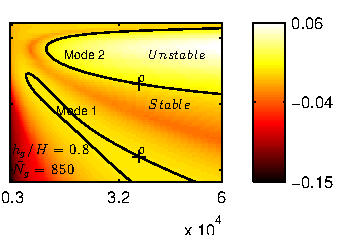
\includegraphics[scale = 0.67]{Set4_dens32_imgsc}} &
{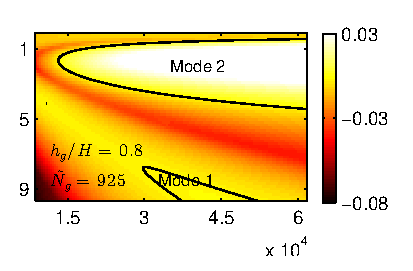
\includegraphics[scale = 0.67]{Set4_dens34_imgsc}} \\
{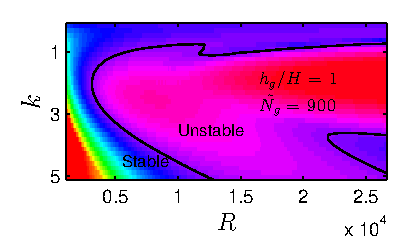
\includegraphics[scale = 0.67]{Set5_dens38_imgsc}} &
{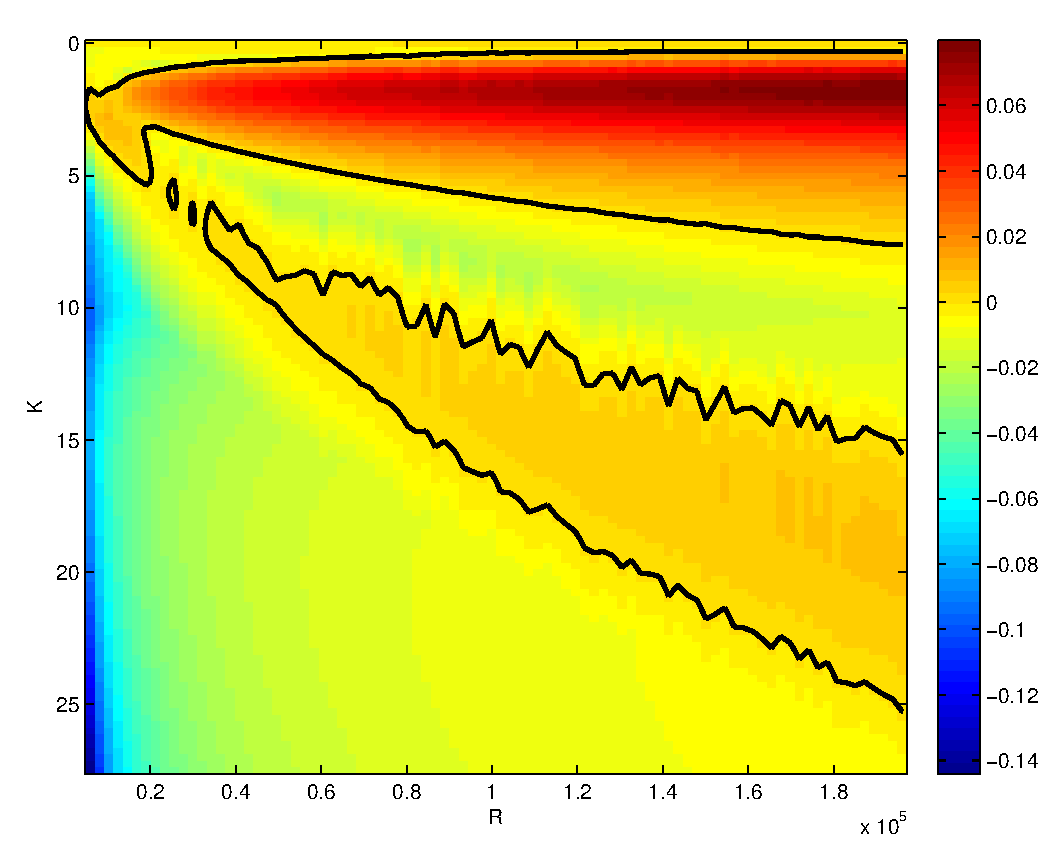
\includegraphics[scale = 0.67]{Set5_dens40_imgsc}} &
{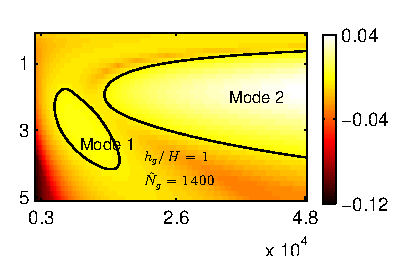
\includegraphics[scale = 0.67]{Set5_dens42_imgsc}} &
{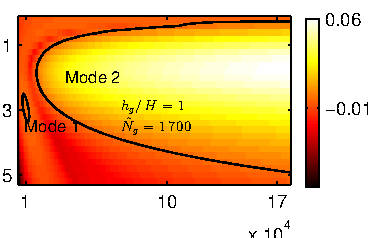
\includegraphics[scale = 0.67]{Set5_dens46_imgsc}} \\
%{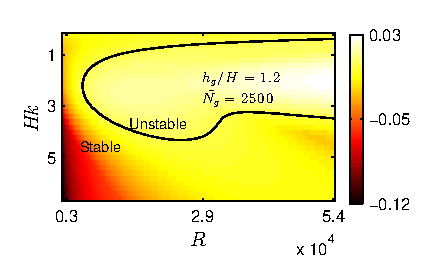
\includegraphics[scale = 0.67]{Set6_dens32_imgsc}} &
%{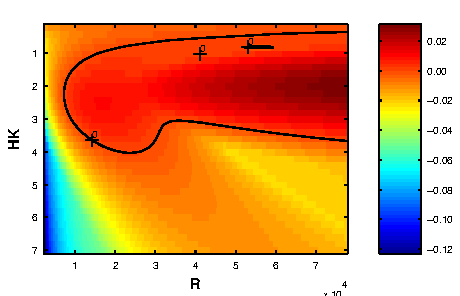
\includegraphics[scale = 0.67]{Set6_dens34_imgsc}} &
%{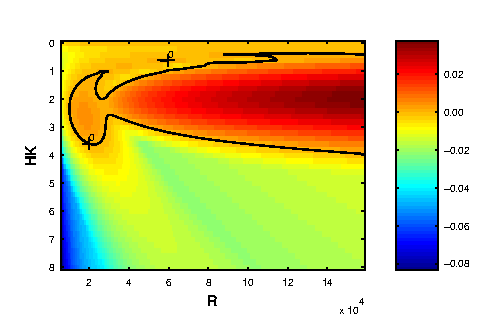
\includegraphics[scale = 0.67]{Set6_dens36_imgsc}} &
%{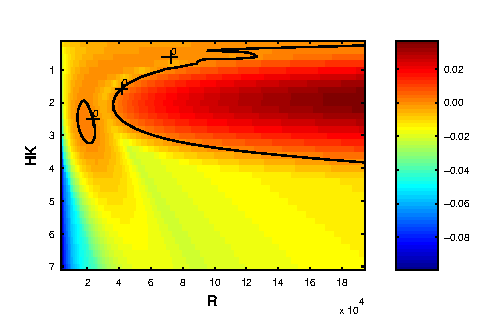
\includegraphics[scale = 0.67]{Set6_dens38_imgsc}}
\end{tabular}
\caption{$Re(\sigma)$ as function of wavenumber and Reynolds number for a specified grass number density $\Ndg$ along with the neutral curve ($Re(\sigma)$=0), for parameters shown in the corresponding panel.  
As $\Ndg \propto N_g$ increases, the unstable region splits into two labeled as ``Mode 1'' and ``Mode 2''. 
For $\Ndg$ below a critical value, the Mode 1 sets the threshold $\Rey$ whereas above the critical $\Ndg$ onset is determined by Mode 2.}
\label{K_Re_sigma_set3}
\end{figure*}

Comparison of frequency (Im$(\sigma)$) of the fastest growing mode with that of experimental observations of frequencies in
the lab scale experiments, for cases where the vegetation was sufficiently dense to be modeled by a continuum drag field, is also shown in the inset in figure \ref{Re_vs_delta}b. 
The observed frequencies are associated with the peaks in velocity spectra, frequency of $\monami$ and frequency of 
vortex passage \cite{Ghisal02}, and compare well with the predicted frequencies. 
%Regardless of the assumptions, the introduction of vegetation drag is observed to damp the linear modes\cite{Delangre06}.

\begin{table*}
\rowcolors{3}{tableShade}{white}  %% start alternating shades from 3rd row
\renewcommand{\arraystretch}{1.4}
 \begin{tabular}{l|c|c|c}
			& Kelvin-Helmholtz 				& Mode 1 		& Mode 2 \\ \hline
 Base velocity profile 	& $U(y) = U_0 \tanh(y/\delta)$			& \multicolumn{2}{c}{$-{dP}/{dx}+\mu U''(y) +S(y) \rho C_N d N_gU^2=0$} \\
 Domain 		& $-\infty < y < \infty$			& \multicolumn{2}{c}{$-1<y<1$} \\
 Inflection point	& exists at $y=0$				& \multicolumn{2}{c}{$U''(y)$ discontinuous at $y=\hg$} \\
 Shear layer thickness	& $\delta$					& \multicolumn{2}{c}{$\delta \sim  H\left(\Rey \Ndg \right)^{-1/3}$} \\
 Linearized dynamics	& $\left(\sigma+ikU\right) \left(D^2-k^2\right)\phi =  ikU_{yy}\phi$		& \multicolumn{2}{c}{Equation \eqref{Orr-somerfield}} \\
 Critical parameters	& none						& $\Rey \propto \Ndg^{1/2}$ 	& $\Rey \propto \Ndg$ \\
 Most unstable $k$ as $\delta \to 0$	& $\propto \delta^{-1}$		& $\propto \delta^{-1}$	& $O(1)$ \\
 Mode localized?	& yes, near $y=0$				& ~~~~yes, near $y=\hg$~~~~			& no
 \end{tabular}
 \caption{Comparison between Kelvin-Helmholtz instability and the two modes resulting from solution of \ref{Orr-somerfield}.}
 \label{tab:comparison}
\end{table*}
To better understand the mechanism of waving and the origin of the threshold, we consider the behavior of the instability as a function of the vegetation drag characterized by $\Ndg$.
The fastest growing wavenumber first increases proportional to $H/\delta$, but at a critical grass density discontinuously jumps and remains $O(1)$ (see figure \ref{Re_vs_delta}). 
To aid in explaining the behavior, we show heat maps of Re$(\sigma)$ as a function of $\Rey$ and $k$, for different $\hg/H$ and $\Ndg$ in figure \ref{K_Re_sigma_set3}. 
The lowest $\Rey$ on the neutral curve sets the threshold. 
We observe that as $\Ndg$ increases, the unstable region splits into two. We refer to the unstable region with the higher $k$ as ``Mode 1'', and the one with the lower $k$ as ``Mode 2''. 
The unstable region for Mode 1, depending on $\hg/H$ either recedes to higher $\Rey$ or shrinks to zero size, as the grass density increases, causing the most unstable mode to jump.

The distinct asymptotic behavior of the two modes as $\Ndg \gg 1$ allows us to understand the mechanism of the instability. 
Mode 1 asymptotically localizes to the boundary layer near the grass tip, and exhibits an asymptotic behavior with $k \sim O(H/\delta)$, and $\Rey \sim (H/\delta)$ (or $\Rey \propto {\Ndg}^{1/2}$) at the threshold. 
This limit can be understood through asymptotically estimating the sizes of the terms in \eqref{Orr-somerfield} using $D\sim \delta^{-1}$, $\sigma \sim \delta^{-1}$, and $U\sim \delta$; the magnitude of the advection term is $\Rey/\delta^3 \sim \Rey^2 \Ndg $, and the viscous term (or the vegetation drag term, which is found to scale identically) in the boundary layer is $\delta^{-4} \sim (\Rey \Ndg)^{4/3}$. 
The terms balance when $\Rey \sim {\Ndg}^{1/2}$ (or $\Rey \sim H/\delta$) leading to a simplification of \eqref{Orr-somerfield} as
\begin{align}
(D^2-k^2)^2 \phi- 2 \Rey \Ndg D( SUD\phi) = \Rey \sigma (D^2-k^2)\phi,
\label{eqn:mode1asymp}
\end{align} 
in a region of thickness O($\delta$) near $y=\hg$.
Since the relative magnitude of the terms on the r.h.s. to those on the l.h.s. of this equation is $\Rey/\Ndg^{1/2}$, we expect identical asymptotic behavior for fixed $\Rey/\Ndg^{1/2}$. Therefore the threshold obtained for Mode 1 is $\Rey \propto \Ndg^{1/2}$ (or $\Rey \propto H/\delta$) explaining the numerically observed asymptote (see figure \ref{Re_vs_delta}). 
This analysis also concludes that the mode structure is self-similar over the length scale $\delta$ for fixed $\Rey/\Ndg^{1/2}$; the verification of this expectation is shown in figure \ref{Asymptotic_mode}, supporting this argument.

On the other hand, the threshold condition for Mode 2 is numerically observed to be $\Rey \propto ({\delta}/{H})^{-3/2}$ (or $\Rey \propto \Ndg$) for $k\sim O(1)$, shown in figure \ref{Re_vs_delta}, which can be understood by an asymptotic scaling analysis of \eqref{Orr-somerfield} by assuming $\Rey \gg 1$ but fixed $\Rey/\Ndg \sim O(1)$.
Note that for large $\Ndg$, the non-dimensional steady flow velocity inside the grass is $U_g \sim (\Rey \Ndg)^{-1/2}$. 
This estimate simplifies \eqref{Orr-somerfield} to 
\begin{align}
\begin{split}
\sigma\left(D^2-k^2\right)\phi = -2{(\Ndg/\Rey)^{1/2}}D^2\phi,  \quad &\text{ for $y<\hg$}  \\
\left(\sigma+ikU\right) \left(D^2-k^2\right)\phi =  ikU_{yy}\phi, \quad &\text{ for $y>\hg$}.
\end{split}
\label{eqn:mode2asymp}
\end{align}
\begin{figure}
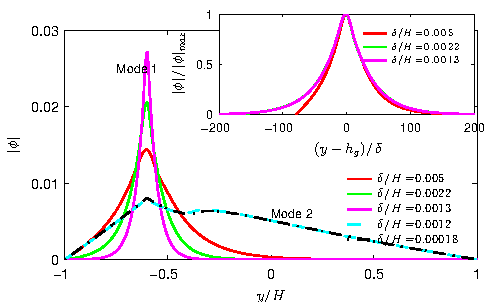
\includegraphics[]{Asymptotic_noshear}
\caption{Plot of mode shape $|\phi|$ for different shear layer thickness in limit of small shear layer thickness for representative values of grass density. 
Mode 1 is shown in solid and Mode 2 is shown in dashed. The parameters Mode 2 shapes are chosen such that $\Rey \gg 1$, $\Ndg \gg 1$ (specified in terms of $\delta/H$) but $\Rey/\Ndg = O(1)$. 
The mode shapes approach each other for these small values of $\delta/H$ indicating that the large grass density asymptote is reached. Mode 1 shapes appear self-similar in shape as $\delta\to 0$, 
and are compared to each other on a rescaled coordinate in the inset. 
Inset shows $|\phi|$ for Mode 1 as a function of $(y-\hg)/\delta$. The modes approach a universal shape, indicating that an asymptotic limit has been reached. 
The limit is not yet reached for the case $\delta/H = 0.005$ due to the influence of bottom boundary; the grass height in this case is comparable to the boundary layer thickness.}
\label{Asymptotic_mode}
\end{figure}
Since $\Rey/\Ndg$ is the only remaining parameter, the mode shape would converge in the aforementioned limit, in agreement with our numerical results for Mode 2 shown in figure \ref{Asymptotic_mode}. 
We interpret Mode 2 as the instability of an inviscid flow, with the vegetation modeled by a continuum drag field, and for which the boundary layer near the grass tip plays no role. The only remaining parameter $\Rey/\Ndg$ 
sets the threshold, leading to the asymptotic behavior $\Rey \propto \Ndg$ (or $\Rey \sim ({\delta}/{H})^{-3/2}$).
%On the other hand, Mode 1 asymptotically localizes to the boundary layer near the grass tip, and exhibits a different asymptotic behavior with $k \sim O(H/\delta)$, and $\Rey \sim (H/\delta)$ (or $\Rey \propto {\Ndg}^{1/2}$) at the threshold. 

%This limit can be understood through asymptotically estimating the sizes of the terms in \eqref{Orr-somerfield} using $D\sim \delta^{-1}$, $\sigma \sim \delta^{-1}$, and $U\sim \delta$; the magnitude of the advection term is $\Rey/\delta^3 \sim \Rey^2 \Ndg $, and the viscous term (or the vegetation drag term, which is found to scale identically) in the boundary layer is $\delta^{-4} \sim (\Rey \Ndg)^{4/3}$. 
%The terms balance when $\Rey \sim {\Ndg}^{1/2}$ (or $\Rey \sim H/\delta$), leading to a simplification of \eqref{Orr-somerfield} as
%\begin{align}
% \begin{split}
%  \text{blah for $y<\hg$} \\
%  \text{blah for $y>\hg$.}
% \end{split}
%\end{align}
%Since, $\Rey/\Ndg^{1/2}$ is the only remaining parameter in this model, explaining the numerically observed asymptote (see figure \ref{Re_vs_delta}). (this language should be improved)
%This analysis concludes that the mode structure is self-similar over the length scale $\delta$; the verification of this expectation is shown in figure \ref{Asymptotic_mode}, supporting this argument.
Table \ref{tab:comparison} compares the two modes to each other, and to the Kelvin-Helmholtz instability. 
Because Mode 1 eigenfunction is localized over a length scale $\delta$, it may be interpreted as the instability of the flow in the boundary layer, whereas Mode 2 may be understood as the instability on the scale of the water column. 
Mode 1 appears to be closely related to the Kelvin Helmholtz mechanism, whereas Mode 2 arises purely from the interaction between the unvegetated water column and the flow through the vegetation. 
Vegetation drag plays a dominant role in the mechanism for both the modes, which distinguishes our analysis from the traditional Kelvin-Helmholtz instability. 
The appearance of vegetation drag parameter in the dominant balances \eqref{eqn:mode1asymp} and \eqref{eqn:mode2asymp}, and the threshold criteria demonstrates its role in setting the threshold.
\newline
Similar phenomenon of large amplitude coherent oscillation of terrestrial canopies in atmospheric flow known as \textit{honami}\cite{Inoue56,Raupach96}, have also been observed.
A crucial difference between the atmospheric and aquatic flow is that the atmospheric flows are essentially unbounded vertically\cite{Vivoni98,Nepf00}. 
Another major difference between the two is the considerable difference of stiffness of canopies; terrestrial canopies tend to be much more rigid, whereas aquatic canopies are buoyant\cite{Vivoni98,Ghisal02}. 
Despite these differences, in the framework of our model, the limit of $\hg/H \ll 1$ while $\delta/\hg$ = constant can be used to represents the hydrodynamic instability for the terrestrial case with stiff grass blades. We find that in this case, the transition from Mode 1 to Mode 2 happens at such a large grass density, so as to make Mode 2 irrelevant. In this manner, we recover the Kelvin-Helmholtz-like characteristics observed in the terrestrial case. 
\newline
The deviation of our model predictions from the observed may be attributed to the various simplification we have made in our model. 
In a real canopy, the drag coefficients are known to vary from bottom to tip of the grass blades\cite{Vivoni98,Nepf00}. 
The turbulent viscosity is also known to vary between the flow of unvegetated region and flow through the canopy\cite{Ghisal02}. 
Although an improved analysis of flow with these variation in the model might lead to a better agreement between the observed and the predicted quantities, these variation are not central to the mechanism leading to the instability of flow.
\newline\newline
In conclusion, we note that the threshold flow condition observed in the field and in lab experiments arises due to the presence of vegetation drag. 
We show the origin of this threshold using a consistent continuum hydrodynamic stabiity analysis for the shear flow that develops as a result of the drag. 
Such an analysis not only explains quantitative observations, but also provides an understanding of the hydrodynamic instability mechanism. 
The extent of the structure of Mode 2 throughout the depth of the water column implies an efficient transport of suspended tracers compared to that due to the localized structure of Mode 1 near the canopy top. 
Our analysis also informs flow structure formation in many other related scenarios, such as flow over coral reefs, permeable sediments, etc. and therefore is expected to have a wider impact.
\bibliography{Grass}{}
\bibliographystyle{plain}
\end{document}
